% =============================================================
% GRAPHICAL ABSTRACT (arquivo separado exigido pelo MethodsX)
% Compilar: pdflatex -output-directory=../build graphical_abstract.tex
% Paineis: recortes reais da sessao da Amazonia, gerados por
% tools/make_ga_crops.py a partir de figures/fig_qualitative.png
% =============================================================
\documentclass[border=6pt]{standalone}
\usepackage{tikz}
\usetikzlibrary{positioning, arrows.meta, calc, decorations.pathreplacing}
\usepackage{xcolor}
\definecolor{gaink}{HTML}{1A5276}
\definecolor{gagray}{HTML}{5A6068}

\begin{document}
\begin{tikzpicture}[
  font=\sffamily,
  panel/.style={draw=black!25, line width=0.4pt, inner sep=0pt},
  gacap/.style={font=\sffamily\small, text=gagray},
  gastep/.style={-{Latex[length=2.6mm]}, line width=1pt, draw=gaink},
]

\newcommand{\pw}{3.5cm}

\node[panel] (a) at (0,0) {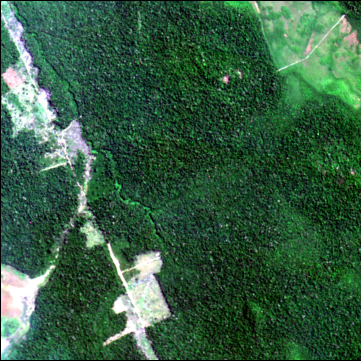
\includegraphics[width=\pw]{ga_before.png}};
\node[panel, right=6mm of a] (b) {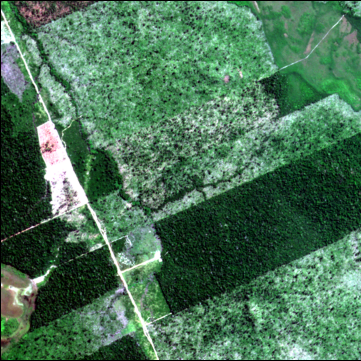
\includegraphics[width=\pw]{ga_after.png}};
\node[panel, right=6mm of b] (c) {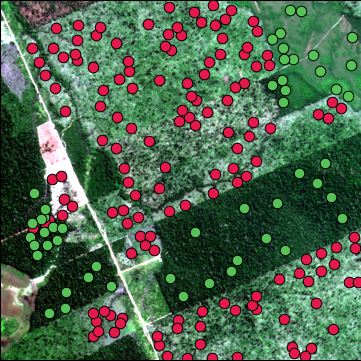
\includegraphics[width=\pw]{ga_clicks.png}};
\node[panel, right=6mm of c] (d) {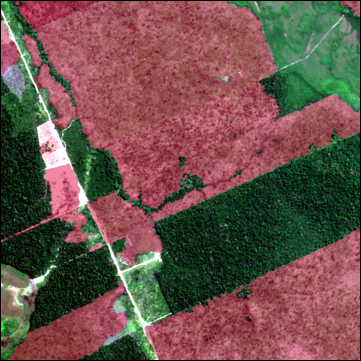
\includegraphics[width=\pw]{ga_pred.png}};

\node[gacap, above=1.5mm of a] {before};
\node[gacap, above=1.5mm of b] {after};
\node[gacap, above=1.5mm of c] {expert clicks on the pair};
\node[gacap, above=1.5mm of d] {predicted change};

\draw[gastep] (b) -- (c);
\draw[gastep] (c) -- (d);

% o par de datas e a unidade de anotacao
\draw[decorate, decoration={brace, mirror, amplitude=4pt}, draw=gagray]
      ($(a.south west) + (0,-2mm)$) -- ($(b.south east) + (0,-2mm)$)
      node[midway, below=4pt, gacap] {one (before, after) pair};

% o ciclo: a predicao volta para o anotador
\draw[gastep] (d.south) -- ++(0,-0.85)
      -| node[gacap, pos=0.25, below] {train, predict, review, click again} (c.south);

\end{tikzpicture}
\end{document}
